\subsection*{Задание}

\begin{enumerate}
\item Для своей программы придумайте минимум 5 тестов. Все 5 тестов необходимо показать при защите.
\item Протестируйте свою программу на этих тестах
\item Можно использовать циклы и условия, но основной частью решения должны быть регулярные выражения.
\end{enumerate}

\begin{figure}[h]
	\centering
	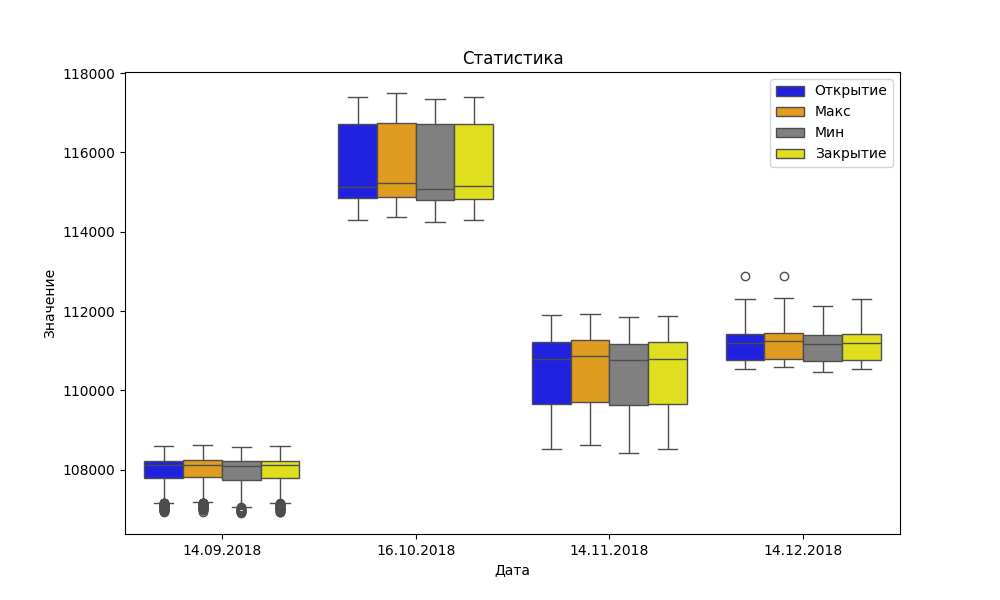
\includegraphics[scale=0.7]{task_3}
\end{figure}

\subsection*{Тестовые файлы}
\subsubsection*{Тест 1}
\textit{Петров П.П. P0000}

\textit{Петров П.П. P3115}

\textit{Анищенко А.Z. P3115}

\subsubsection*{Тест 2}
\textit{Сидоров С.С. P3115}

\textit{Петров П.П. P3114}

\textit{Васильев В.И. P3115}

\subsubsection*{Тест 3}
\textit{Кузнецов А.А. P3115}

\textit{Лебедев К.Н. P3116}

\subsubsection*{Тест 4}
\textit{Сафонов С.Ю. P3115}

\textit{Соловьев В.А. P3115}

\subsubsection*{Тест 5}
\textit{Романов Р.С. P3115}

\textit{Попов П.П. P3115}

\subsection*{Листинг}
\begin{minted}[breaklines]{python}
import re
from pathlib import Path

GROUP = "P3115"

TEXTS_PATH = Path(__file__).parent / "texts" / "task_3"
PATTERN = re.compile(
    r"^(\w)\w+\s+(?:\1(?:\.|\w+\s+))+\s+{group}$".format(group=GROUP),
    flags=re.IGNORECASE | re.MULTILINE
)

CORRECT_ANSWERS = (
    "Петров П.П. P0000\nАнищенко А.Z. P3115",
    "Петров П.П. P3114\nВасильев В.И. P3115",
    "Кузнецов А.А. P3115\nЛебедев К.Н. P3116",
    "Сафонов С.Ю. P3115\nСоловьев В.А. P3115",
    "Романов Р.С. P3115"
)


def find_words(text: str) -> set[str]:
    return set(PATTERN.findall(text))


def main() -> None:
    for i in range(1, 6):
        text = (TEXTS_PATH / f"text_{i}").read_text(encoding="utf-8")
        processed_text = PATTERN.sub("", text).strip()
        processed_text = re.sub(r"\n{2,}", "\n", processed_text)
        correct_answer = CORRECT_ANSWERS[i - 1]

        if processed_text != correct_answer:
            print(
                f"Ошибка в тесте {i}\n"
                f"Ожидалось - {correct_answer}\n"
                f"Результат - {processed_text}"
            )
        else:
            print(f"Текст {i}: результат - {processed_text}")
            print("=" * 100)



if __name__ == '__main__':
    main()
\end{minted}

